\documentclass[a4paper,14pt]{extarticle}
\usepackage{geometry}
\usepackage[T2A]{fontenc}
\usepackage[utf8]{inputenc}
\usepackage[french, russian, english]{babel}
\usepackage{amsmath}
\usepackage{amsthm}
\usepackage{amssymb}
\usepackage{fancyhdr}
\usepackage{setspace}
\usepackage{graphicx}
\usepackage{colortbl}
\usepackage{tikz}
\usepackage{pgf}
\usepackage{subcaption}
\usepackage{listings}
\usepackage[colorlinks, linkcolor=blue, urlcolor=blue]{hyperref}
\usepackage{indentfirst}
\graphicspath{{images/}}


\makeatletter
\renewcommand{\@biblabel}[1]{#1.} 
\makeatother

\geometry{left=2.5cm}
\geometry{right=1.5cm}
\geometry{top=1.5cm}
\geometry{bottom=1.5cm}
\renewcommand{\baselinestretch}{1.5}

\newcommand{\bibref}[3]{\hyperlink{#1}{#2 (#3)}}

\renewcommand{\theenumi}{\arabic{enumi}}% Меняем везде перечисления на цифра.цифра
\renewcommand{\labelenumi}{\arabic{enumi}}% Меняем везде перечисления на цифра.цифра
\renewcommand{\theenumii}{.\arabic{enumii}}% Меняем везде перечисления на цифра.цифра
\renewcommand{\labelenumii}{\arabic{enumi}.\arabic{enumii}.}% Меняем везде перечисления на цифра.цифра
\renewcommand{\theenumiii}{.\arabic{enumiii}}% Меняем везде перечисления на цифра.цифра
\renewcommand{\labelenumiii}{\arabic{enumi}.\arabic{enumii}.\arabic{enumiii}.}% Меняем везде перечисления на цифра.цифра

\newcommand{\imgh}[3]{\begin{figure}[h]\center{\includegraphics[width=#1]{#2}}\caption{#3}\label{ris:#2}\end{figure}}

\begin{document}
	\begin{titlepage}
\newpage

\begin{center}
Федеральное государственное автономное образовательное учреждение высшего образования "Национальный исследовательский университет "Высшая школа экономики"
\\
\medskip
Факультет компьютерных наук \\
Основная образовательная программа \\
Прикладная математика и информатика \\
\end{center}

\vspace{8em}

\begin{center}
\Large КУРСОВАЯ РАБОТА \\
\end{center}

\vspace{2em}

\begin{center}
\textsc{\textbf{
Исследовательский проект на тему
\linebreak
"Оценка неопределенности для Машинного Перевода"}}
\end{center}

\vspace{6em}



\newbox{\lbox}
\savebox{\lbox}{\hbox{Ментимер Шаймиев Рудольф Нуриев}}
\newlength{\maxl}
\setlength{\maxl}{\wd\lbox}
\hfill\parbox{17cm}{
\hspace*{5cm}\hspace*{-5cm}Выполнил студент группы 171, 3 курса: \hfill Кузнецов Дмитрий Сергеевич\\
\hspace*{5cm}\hspace*{-5cm}Руководитель КР\hfill 
научный сотрудник Лобачева Екатерина Максимовна\\
%\hspace*{5cm}\hspace*{-5cm}Куратор:\hfill < степень>, <звание>, <ФИО полностью>\\
}


\vspace{\fill}

\begin{center}
Москва 2020
\end{center}

\end{titlepage}% это титульный лист
	\newpage

	{
		\hypersetup{linkcolor=black}
		\tableofcontents
	}

	\newpage
	
	\section{Annotation}
	In the field of machine translation \textit{beam search} is the one of the main methods for improving the quality of the final prediction. However, when using neural network technologies, there is a problem of larger beam size, which limits the richness of beam search. Problem solution will significantly improve the quality of predictions by considering more hypotheses in the process of making predictions. Many factors in the model infrastructure can cause the appearance of the beam problem. In this paper we explore the \textit{larger beam size problem} and its correlation with \textit{model uncertainty}. We also study the propensity of models with an uncertainty estimation to cause beam problem.
	
	\section{Keywords}
		machine translation, uncertainty estimation, beam search, larger beam size problem, model uncertainty
		
	\section{Introduction}
	Note that in the example, some features of the model lead to a bad translation. Our model gave low probable in general predictions as a result under the influence of certain factors. \textit{Uncertainty} can cause such phenomena, in particular \textit{model uncertainty}, the uncertainty of predictions caused by the model. What if we can construct some probability measure on the space of output sentences $f_1, \dots, f_m$. In this case, we will be able to estimate in total how much it is typical to get a particular prediction and adjust the output of the model. The task of explicitly or implicitly constructing such a distribution on outputs is called \textit{uncertainty estimation}.
	
	There are articles that consider different types of uncertainties and their impact on beam search. In this paper, we investigate the influence of model uncertainty on the beam problem. We also investigate the applicability of the uncertainty estimation methods in the neural machine translation problem and their impact on the effectiveness of beam search.
	
	\section{Machine Translation}
	\subsection{Preliminary}
		The task of machine translation is to provide a sentence equivalent in meaning in the target language for the original sentence in the source language. Let $e_1, \dots, e_n$ be a sequence of input sentence tokens' vector representation in the source language. The machine translation model is required to build a sequence of tokens $f_1, \dots, f_m$ in the target language, moreover, in this language, this sequence must have the original meaning.
	
	Most modern neuromachine translation models follow the paradigm \bibref{seq2seq}{Sutskever et al.}{2014} (seq2seq). Seq2seq models often consist of two recurrent neural networks or groups of networks. One network that processes input tokens is called \textit{encoder}, the second network that builds output predictions is called \textit{decoder}. The encoder task is to encode the input sequence into some hidden representation $h_1, \dots, h_p$, which is fed to the decoder as hidden initialization before building the output prediction. The decoder output is a vector set $\{(p_{i1}, \dots, p_{id})\}_{i=1}^{m}$, where $d$ - target language dictionary power, $m$ - maximum possible prediction sequence length, $p_{ij}$ - the model's confidence that the $i$th token of the predicted sentence will be the $j$th token from the target language dictionary. As a result, the translation model builds a "probability distribution" in the space of the cartesian product of the target dictionary.

	The simplest and most obvious way to build a prediction (final translation) is to select the token that the model is most confident in at each step. If $f_1, \dots, f_m$ is a sequence of model hypotheses' tokens, then $f_i := argmax \, \{p_{ij}\}_{j=1}^{d}$. However, for an optimal prediction $f_1^*, \dots, f_m^*$ it is not always true that in terms of model confidence $f_i^* = argmax \, \{p_{ij}\}_{j=1}^{d}$. This phenomenon is also related to the beam problem, which we will discuss in more detail in the following chapters.
	\subsection{Statement}
	В первую очередь, определим понятие эмбединги. Эмбединги - это некоторые численные вектора специального векторного пространства, которые взаимнооднозначно соответствуют словам из словаря некоторого языка. Тогда рассмотрим следующую постановку.
	Пусть $\textbf{x}, \textbf{r}$ - эмбединги, соответствующие входным и выходным токенам $\textbf{e}, \textbf{f}$, соответственно. 
	Тогда модель машинного перевода задает следующую куммулятивную вероятность:
	\begin{equation}
		P(\textbf{y} | x, \theta) = P(y_1 | x, \theta) \prod_{i=2}^{L} P(y_i | y_{<i}, \textbf{x}, \theta)
	\end{equation}
	
	Здесь $\textbf{y}$ - некоторая последовательность токенов, которая соответствует переводу с точки зрения модели. $y_{<i}=(y_1, \dots, y_{i - 1})$, а $\theta$ - параметры модели машинного перевода, настраиваемые в процессе обучения.
	
	На основе данных вероятностей модель в дальнейшем выбирает по некоторому правилу итоговую последовательность эмбедингов  $\textbf{y} = (y_1, \dots, y_m)$ и по ним однозначно восстанавливает итоговые токены $\textbf{h} = (h_1, \dots, h_m)$. Как мы уже рассмотрели ранее, в качестве решающего правила может выступать жадный выбор, т.е. на каждой итерации выбирается эмбединг с максимальной условной вероятностью $P(y_i | y_{<i}, \textbf{x}, \theta)$, либо в качестве решающего правила можно использовать некоторый другой подход, например, beam search, который мы рассмотрим далее.
	
	Для простоты в силу взаимнооднозначности далее под токенами будем понимать эмбединги токенов и будем неявно подразумевать перевод в пространство итоговых токенов. Поэтому конечными нашими обозначениями будут: $X = (x_1, \dots, x_n)$ - множество всех предложений на исходном языке, $R = (r_1, \dots, r_n)$ - множество истинных переводов на целевом языке. $Y = (y_1, \dots, y_n)$ - множество переводов с точки зрения нашей модели.
	
	Наиболее часто встречаемой мерой качества в задаче машинного перевода является BLEU. 
	
	Пусть модель для некоторой пары предложений $\textbf{x}, \textbf{r}$ построила перевод $\textbf{y}$.
	\begin{equation}
		BLEUK = \min\Big(1, \, \frac{|\textbf{y}|}{|\textbf{r}|}\Big) \big(\prod_{i=1}^{K} precision_i\big)^{\frac1K}
	\end{equation}
	
	Здесь под $precision_i$ понимается $precision$ посчитанный по всем i-граммам.
	\section{Beam Search}
	\subsection{Motivation}
	Beam search is used as a more effective solution for building predictions. Its main idea is that instead of selecting the most likely token at each step, we require the model to store $b$ the most likely predictions' prefixes $y_{b1}, \dots, y_{bt}$. Using this approach, we do not choose the locally optimal token, but in general the optimal prefix, which will increase the chances of building a correct prediction.

	It is easy to understand that with the increase of $b$ (this hyperparameter is called \textit{beam size}), the quality of the prediction should also increase, since the number of greedy searches is growing. In practice, it turns out that in neuromachine translation, starting from a certain threshold, the quality decreases significantly with increasing beam size. An illustration of this phenomenon can be seen in Fig. 1. The model used in the experiment is described in the  \bibref{fconv}{Jonas Gehring}{2017}. 
	
	\begin{figure}[t]
		\center{
			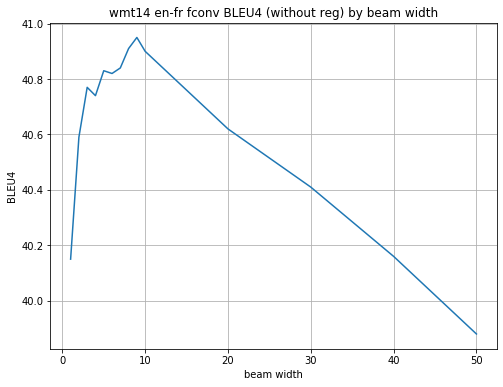
\includegraphics[width=0.7\textwidth]{fconv-bleu4.png}
		}
		\center{\caption{Convolutional Sequence to sequence model BLEU4 evaluation by beam size. Training set: \textit{WMT'14 English-France}}}
	\end{figure}
	
	This problem is called \textit{larger beam size problem}. Next, we will look at the possible causes of this phenomenon in details, until we note that the following situation is not excluded. Suppose on $k_1$ iteration step beam search stores the prefix $y_1, \dots, y_{k_1}$ among $b$ locally optimal, which has the least model confidence among all $b$ prefixes. Let this prefix be constructed in such a way that on the next steps model will find a suffix that complements it in such a way that the final sentence is considered the optimal translation from the model's point of view. There are cases when such a translation can be incorrect. Consider following example. Let us train a translation model on a fairy tale corpus, the source language is Russian and the target language is English. Consider the following sentence: \textit{Жульничество на экзамене однажды может закончиться проблемами}. Suppose following sentence is a model prediction: \textit{At the examination once upon a time}. It is obvious that the meaning of the translation does not correspond to the original sentence, but this sentence is optimal from the point of view of our hypothetical model. Beam problem can cause such situations. The prefix \textit{At the examination once} may have been included in a broad beam search and have been earned a low model confidence. However, due to the fact that we train on a large corpus of fairy tales, where there are many examples of sentences like \textit{Once upon a time...} our model decides that after \textit{Once} it is probably to continue prefix with suffix \textit{upon a time}, which lead to a bad translation.
	\subsection{Method definition}
	Suggest $k$-long prediction prefix:
	\begin{equation}
		y_{<k}^{i} := (y_1^{i}, \dots, y_k^{i}) \text{, \,\, where i - beam search branch index}
	\end{equation}
	
	Let us introduce following iterative method:
	
	\begin{enumerate}
		\item Let us submit a special token of the beginning of the sentence and the encoder hidden state to the decoder input. We get a certain tokens' confidence vector $(p_1^{00}, \dots, p_d^{00})$, where $d$ - target dictionary power.
		
		\item Take tokens whose confidence values are $beam$ highest among $ (p_1^{00}, \dots, p_d^{00})$. Here $beam$ is the hyperparameter of the method and is called \textit{beam size}. As a result, we will remember: $y_{<1}^1, \dots, y_{<1}^{beam}$. 
		
		\item In the next iteration, we will submit to the decoder $(y_1^{00}, \dots, y_d^{00})$ as inputs and the hidden state of the previous step. For each token, we get our output distribution $(p_1^{1i}, \dots, p_d^{1i})$ (here $1$ is the iteration number, $i$ is the token number).
		\item For all token $i \in \overline{1, beam}$ consider $\forall j \in \overline{1, d}: \,\, p(f_{:1}^i) * p_j^{1i}$. We get a set of prefixes of length $2$. Let us choose among all $beam * d$ prefixes $beam$ with the greatest confidence. Remember them: $y_{<2}^1, \dots, y_{<2}^{beam}$
		
		\item Iteratively, we will continue the operation $\forall k \in \overline{3, m}$. 
		
		We will get: $y_ {<k}^1, \dots, y_{<k}^{beam}$
		
		\item As the final prediction select $y_{<m}^i, \dots, y_{<m}^i$ such that its confidence is greatest $\forall i \in \overline{1, beam}$
	\end{enumerate}
	
	In summary, this method stores $beam$ of the "most likely" prefixes at each decoding iteration, in contrast to the naive approach, which greedily selects 1 locally optimal hypothesis at each iteration.
	
	\subsection{Large Beam Size Problem}
	In General, in neuromachine translation tasks large beam size problem is a phenomenon, as a result of which, starting from a certain threshold value, the quality metric decreases with the growth of the beam size. In this section, we will look at some approaches that do not solve the problem completely, but significantly reduce the effect of metric degradation.
	
	The article \bibref{corr_len_bias}{Murray et al.}{2018} raises two issues: the beam problem and the tendency of NMT models to make short predictions. According to the author, solving the short prediction problem involves solving the beam problem.
	
	As a demonstration of the reasons listed in this article that cause the beam problem, consider the following example from the article.
	
	On the Fig.2. we can see a tree of Beam Search predictions for the word \textit{un hélicoptère}. Let the size of the beam search be 2 and on the first iteration we saved two hypotheses: \textit{a} and \textit{an}. Note that all 4 following hypotheses can be potential translation options, but \textit{a helicopter} in this example is a correct translation. However, \textit{autogyro} is an only one continuation for prefix \textit{an}, thefore the model confidence for this suffix is $1$, and as a result, the model confidence to predict \textit{an autogyro} is equal to $0.4$. At the same time, the probability mass for the \textit{a} continuation suffixes is divided among the words: \textit{helicopter, chopper, whirlybird}. As a result, the confidence for the correct translation of \textit{a helicopter} from the model's point of view is $0.36$. As a result, the model will give a bad prediction. Larger beam size we take, higher probability we get in this situation, hence the loss of quality.
	
	\begin{figure}[t]
		\center{
			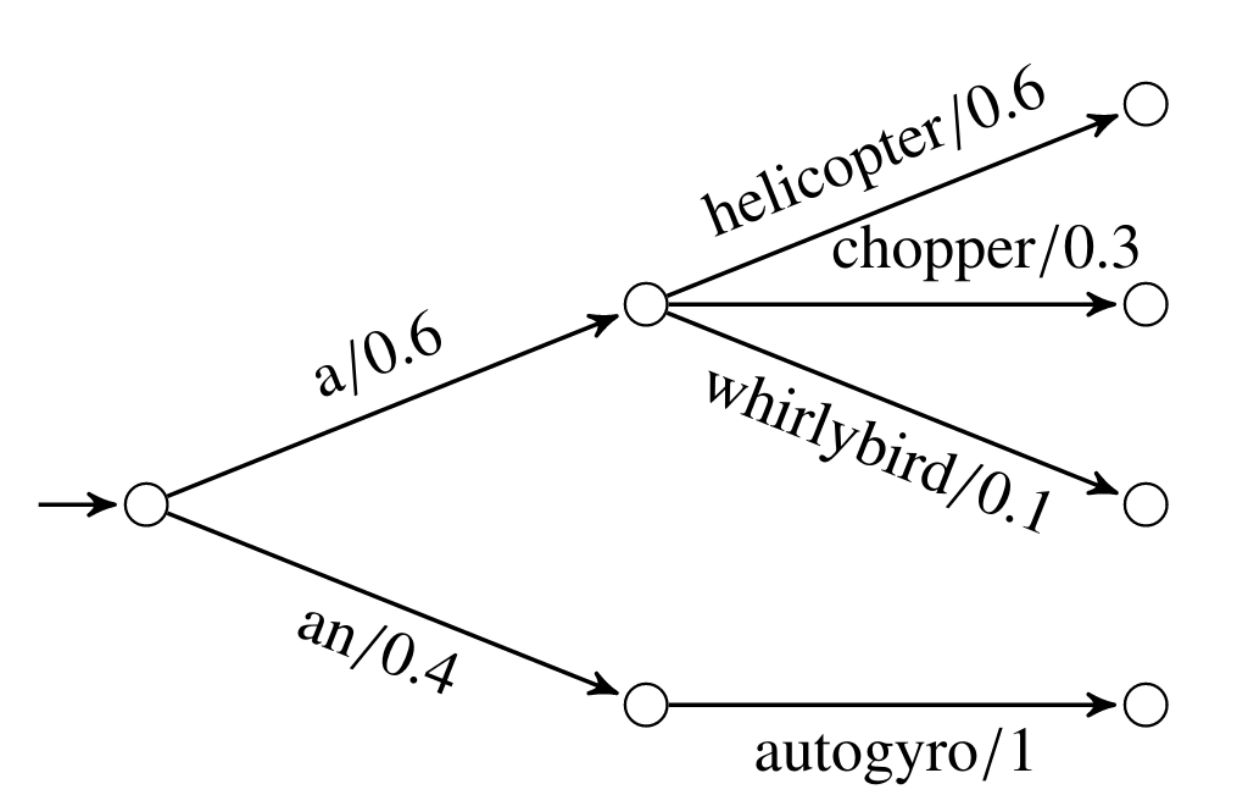
\includegraphics[width=0.5\textwidth]{helicopter.png}
		}
		\center{\caption{Label bias causes this toy word-by-word translation model to translate French helicopter incorrectly. This figure is taken from [4].}}
	\end{figure}
	
	Note that this example demonstrates the fact that if a certain prefix involves a low-entropy suffix, the model tends to ignore the second input token and predict with high confidence one of several highly probable low-entropy suffixes. As a result, the low entropy of the suffix leads to overestimation of this prediction branch and as a result, poor quality. In addition, there is a high probability of getting short predictions due to low entropy, since the model begins to ignore some tokens in favor of high confidence of low-entropy suffixes. For this reason, the authors of the article consider the short prediction problem and the beam problem together.
	
	Standard quality functional for a machine translation task is \textit{cross-entropy}:
	\begin{equation}
		s(\textbf{y}) = \sum_{i=1}^{L}\log p(y_i | y_{<i}, \textbf{x}, \theta), \,\,\, \text{where $L$ - translation length}
	\end{equation}
	
	The authors consider the following quality functional adjustments as solutions:
	\begin{enumerate}
		\item Length normalization
		\begin{equation}
			s'(\textbf{y}) = s(\textbf{y}) / L
		\end{equation}
		
		\item \bibref{gnmt}{Google's NMT system}{2016}. Length normalization. 
		\begin{equation}
			s'(\textbf{y}) = s(\textbf{y}) \Big/ \frac{(5 + L) ^ \alpha}{(5 + 1) ^ \alpha}
		\end{equation}
		
		\item Word reward
		\begin{equation}
			s'(\textbf{y}) = s(\textbf{y}) + \gamma L
		\end{equation}
	\end{enumerate}
	
	Let us look at the results presented in the article for the \textit{WMT'17 Russian-English} model. The architecture presented in the article \bibref{encdec_att}{Bahdanau et al.}{2015} was chosen as the baseline. Appealing to experiments results from the paper we observe that the solution of the short prediction problem using methods proposed above significantly decreases the influence of the beam problem on the considered dataset. Comparing \textit{word reward} and {length normalization}, we can see that they earn quite close BLEU values and lager beam size problem affects models in a same way, when baseline model suffers from beam problem significantly.
	
	Let us now look at the article \bibref{six_chall}{Koehn et al.}{2017}. This is a review article on the main problems of neuromachine translation, including the beam problem.
	
	The authors of the article do not present new solutions for the problem, but conduct a review study. As a baseline, they use the same neural network as in the previous article: attention-based encoder-decoder. Fig. 3 presents their results for various \textit{WMT} datasets. Here, normalization is the Length normalization from the previous article.
	
	\begin{figure}[t]
		\center{
			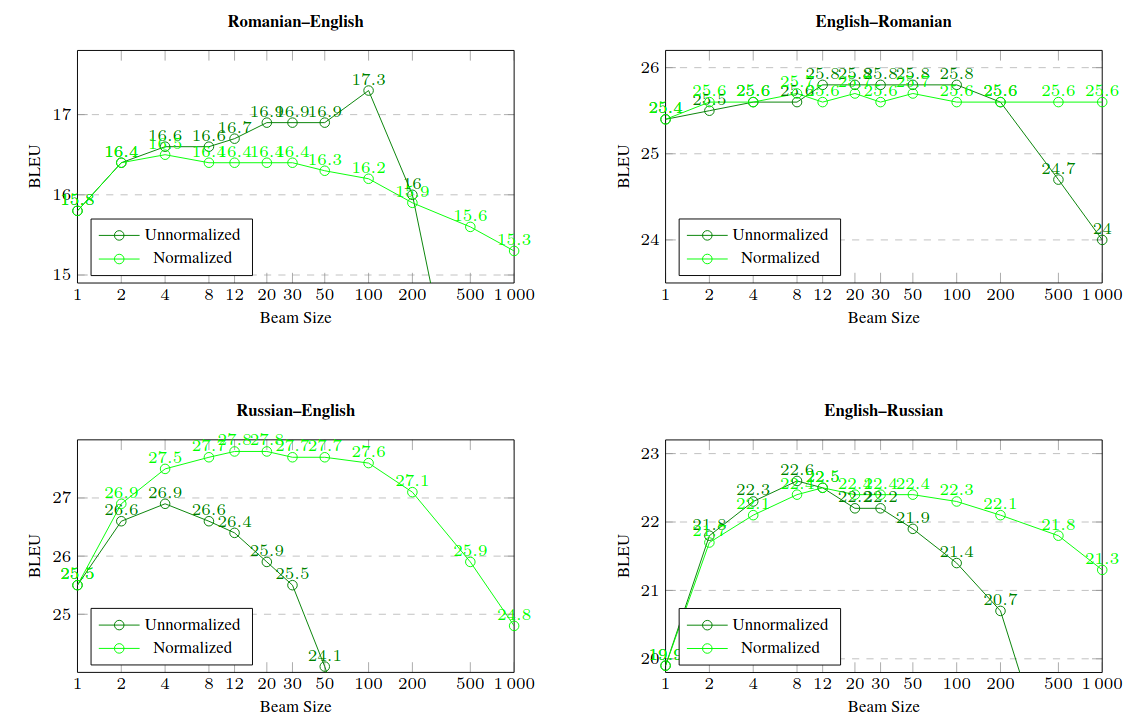
\includegraphics[width=0.8\textwidth]{six_chall_graph.png}
		}
		\center{\caption{Translation quality with varying beam sizes. For large beams, quality decreases, especially when not normalizing scores by sentence length. This figure is taken from [7].}}
	\end{figure}
	
	The results obtained in this article are consistent with the results and conclusions of the previous article.
	
	Consider an article that offers a different method for solving the problem \bibref{calibration}{Kumar et al.}{2019}.

	In this article the beam problem solution is based on the calibration of the probability distribution $p_{it}: = p(y_{i, t} | y_{i,<t})$, here $i$ is the index of the sample example. Before starting the review, let us introduce the definition of "well-calibrated" distribution. Output distribution $p (y_{i, t} | y_{i, <t})$ \textit{well calibrated} if:
	\[
		\forall \beta \in [0, 1]: \frac{ | \{ y \in V |\, p(y) = \ beta \} | }{d}=\beta
	\]
	where V is the target language dictionary.
	
	Let us denote calibration metrics \textbf{expected calibration error (ECE)}:
	
	Let $\mathbf{r}_i = (r_{i1}, \dots, r_{im})$ be reference sentece $\mathbf{x}_i$.
	
	Model predictions: $\mathbf{y}_{it} := argmax_{y} p(y | y_{i, <t})$.
	
	$C_{it}(f) := \delta(r_{it} = y)$, where $\delta$ - Kronecker delta.
	
	Let us divide probability space $[0, 1]$ by $M$ equal bins: $I_1, \dots, I_M$.
	
	Let $L = \sum_i^N |\mathbf{r}_i|$ be a total output token length.
	
	Then:
	\begin{equation}
		ECE = \frac1{L}\sum_{b=1}^{M}\Big|\sum_{i, t:\, p(\mathbf{y}_{it}) \in I_b} C_{it}(\mathbf{y}_{it}) - p(\mathbf{y}_{it})\Big|
	\end{equation}
	
	The reasons why the probability distribution calibration can solve problems with beam size follow from the examples we discussed above.
	
	The authors consider the classic \textit{temperature scaling as the basic method}:
	
	The method is quite simple. It is necessary to raise all probability distribution to the power of $\frac1{T}$, where $T$ is the hyperparameter of the method:
	\[
		p_{it} \rightarrow p_{it}^{\frac1{T}}
	\]
	
	This approach does not change the relative values of probabilities, i.e. it does not locally change the optimality of a particular choice, but it helps to smooth out the consequences of overestimating or underestimating certain prefixes or suffixes.
	
	The authors consider 3 models trained on \textit{WMT} as a baseline: \bibref{encdec_att}{attention-based encoder-decoder}{2015}, GNMT \bibref{gnmt}{Wu et al.}{2016}, transformer \bibref{transformer}{Vaswani et al.}{2017}. Authors build probability plots for each model output distribution with and without classic temperature scaling. Results show that transformer model output distribution is closer to perfect calibration than other models, even without scaling. Classic attention-based encoder-decoder, trained on English-Vietnamese WMT dataset, shows the worst calibrated output distribution without using temperature scaling. Other model in a list, trained on other sets of data, shows quite similar results without calibration method and with temerature scaling, this results differ a little from transformer values. Graphs show that using classic temperature scaling probability plot goes to perfect, ECE decreases even in the worst case scenarios. 
	
	In order not to overweight the literary review, we will not formally introduce the method proposed by the authors. We will consider conceptual differences from the default temperature scaling. To study the formal definition of the method, you can refer to the article \bibref{calibration}{Kumar et al.}{2019}.
	
	As a result of experiments, the authors found out that end of sequence (EOS) token probability is the worst calibrated among all other tokens. Therefore, first of all, the authors calibrate the distribution of the EOS token. This observation strongly correlates with the conclusions from the articles reviewed earlier. In contrast to the classic temperature scaling and the hyperparameter selection on a validation set, the authors propose to make the hyperparameter flexible, different for each example and token index, i.e. not to smooth the entire probability mass, but to smooth it depending on the offset of the probability density on the token. To find the values of hyperparameters, it is proposed to use two fully connected two-layer neural networks with 3 neurons on the hidden layer. The composition of two neural networks with optimization \textit{Negative Log Likelihood (NLL)} is proposed to train to predict the value of the hyperparameter $T$ for a given example and a token in the prediction.
	
	Authors present experiments results, that comparing ECE and BLEU for baseline models with authors calibration method, classic temperature scaling and without any calibration. In generall we can say that temperature scaling gives significant fall comparing to models without any calibration (about several points of number). Authors' calibration method shows the best results except only one case, ECE of output distribution is less than ECE of temperature scaling models (about several points of number after the dot). It can also be seen that the authors' calibration method achieves the best results on the most part of the baseline models from the BLEU point of view.
	
	Now, turning to Fig. 4, let us look at the effect of the authors' calibration on the beam size problem. It is easy to see that calibration significantly reduces the impact of the beam problem.
	
	\begin{figure}[t]
		\center{
			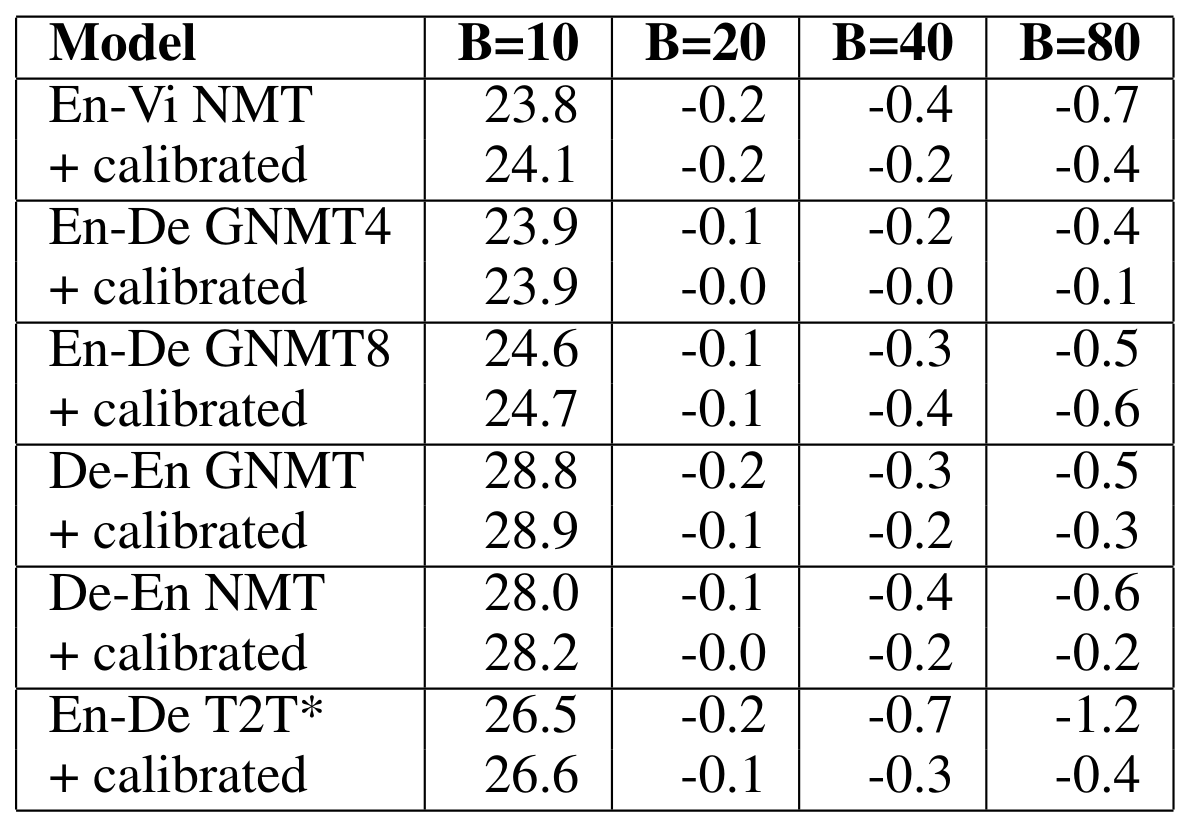
\includegraphics[width=0.6\textwidth]{beam_calibration.png}
		}
		\center{\caption{BLEU with increasing beam on the devset. *Beam sizes for Transformer/T2T: 4, 8, 10 and 12. This figure is taken from [8].}}
	\end{figure}
	
	In this section, we investigated the possible causes of the beam problem, as well as methods of counteraction. Unfortunately, it is not possible to draw unambiguous conclusions from the results of the article about which method shows the best results due to the fact that the experiments in the articles were carried out in different configurations. According to approximate estimates, both methods show good results, are easy to implement, but do not solve the problem completely.
	
	In the next section, we look at a different view of the beam problem, from the perspective of uncertainty.
	
	\section{Uncertainty}
	\subsection{Definition}
	This information was obtained from the article \bibref{prior}{Malinin et al.}{2018}
	
	Uncertainty in machine learning is usually understood as a measure of the nondegeneration of the distribution on the model predictions at a fixed input. Less formally, if we were able to estimate uncertainty, we could tell how much we can trust the model's predictions.
	
	There are several types of uncertainties: data uncertainty, model uncertainty, and distributive uncertainty. \textit{Data uncertainty (aleatoric uncertainty)} - type of uncertainty caused by the nature of the data, including noise, class balance, etc. \textit{Model uncertainty (epistemic uncertainty)}  measures uncertainty caused by a model specifity, how good a model understands given data. \textit{Distributional uncertainty} measures similarity between training and test data, caused by unknown or strange test examples. 
	
	It is important for the model to evaluate all types of uncertainty, because they are caused by different reasons and have different negative effects.
	
	\subsection{Analyzing Uncertainty in Neural Machine Translation}
	In the article \bibref{anal_uncertainty}{Ott et al.}{2018} \textit{data uncertainty} is being investigated.
	
	Let us introduce several base definition from the article. \textit{Intrinsic uncertainty} is the result of existence of several semantically equivalent translations of the same source sentence, for instance there are several ways to express the same meaning. Also situations when target language is more complex than a source language, it can cause an uncertainty. In such situations it could be impossible to earn additional information, such as gender or tense, which is necessary to build correct prediction in a source language. Web data crawling to construct train corpus can cause \textit{extrinsic uncertainty}. For example, authors notice that at least 1\% sentences in WMT datasets is just a copy of a source sentences.
	
	The architecture described in the article \bibref{fconv}{Gehring et al.}{2017} is specified as the baseline of the experiments.
	
	One of the main problems that is raised in this article is an effect of \textit{uncertainty} on the degradation of quality with the growth of beam size. Authors notices copies (extrinsic uncertainty) are overrepresented in the output of beam search. Also they say that bigger beam size we take, more copies appear in a beam search tree, and this growth is quite significant.
	
	\begin{figure}[t]
		\center{
			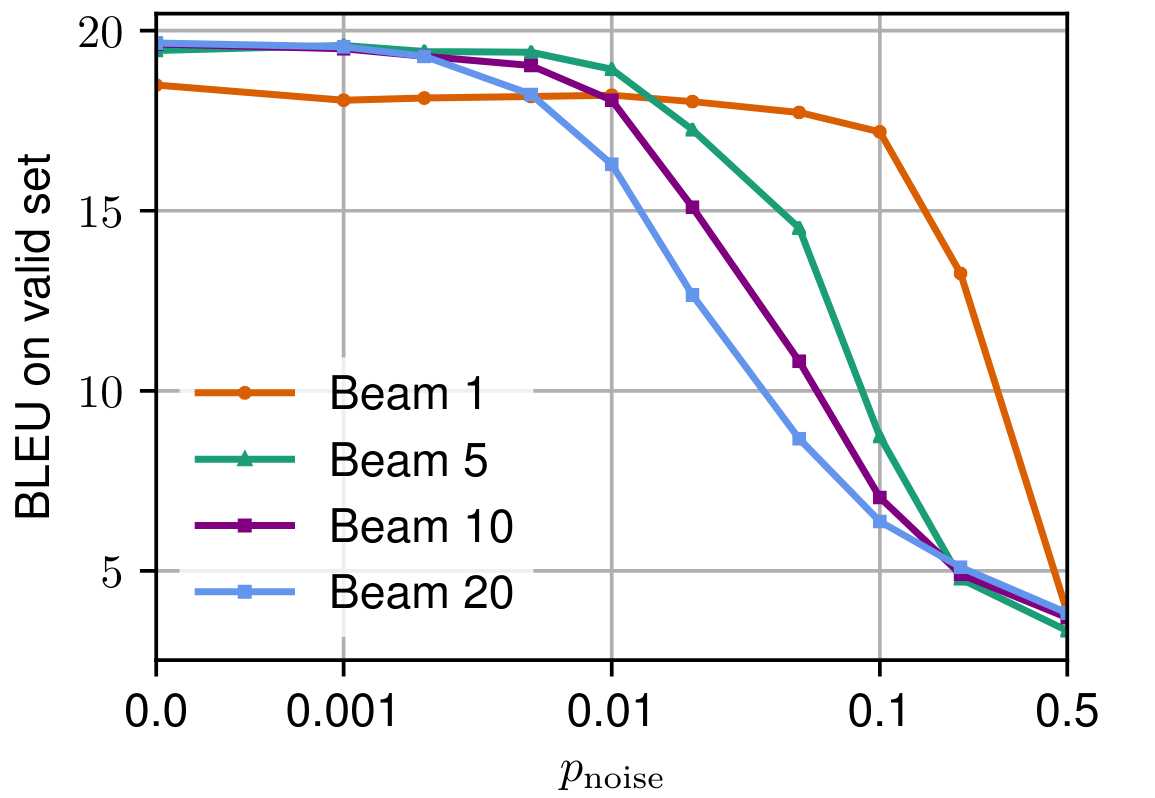
\includegraphics[width=0.6\textwidth]{unc_beam_noise.png}
		}
		\center{\caption{Translation  quality  of  models  trained  on  WMT’17 English-German news-commentary data with added synthetic copynoise in the training data (x-axis) tested with various beam sizeson the validation set. This figure is obtained from [9].}}
	\end{figure}
	
	\begin{figure}[t]
		\center{
			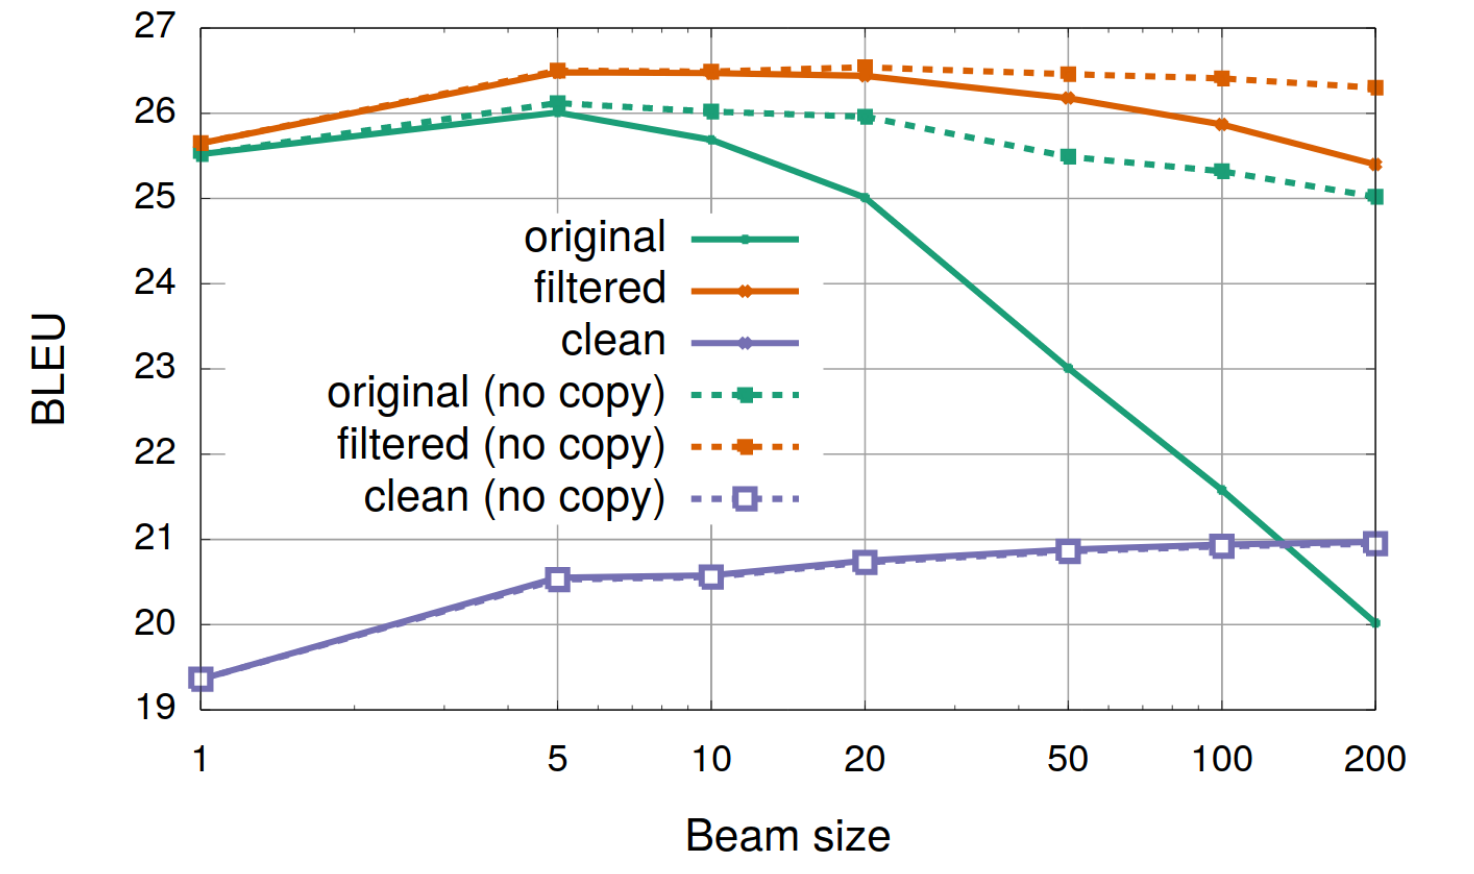
\includegraphics[width=0.6\textwidth]{unc_beam_meth.png}
		}
		\center{\caption{BLEU on newstest2017 as a function of beam width for models trained on all of the WMT’17 En-De training data (original), a filtered version of the training data (filtered) and a small but clean subset of the training data (clean). They also show results when excluding copies as a post-processing step (no copy). This figure is obtained from [9].}}
	\end{figure}
	
	The authors conducted an experiment, the results of which can be seen in Fig. 5, in which WMT'17 added explicitly replaced random examples from the training with copies of the original sentence. It is clearly seen that this leads to quality degradation with increasing noise. Moreover, models with a larger beam size suffer more from extrinsic uncertainty, which confirms the thesis put forward in the previous paragraph.
	
	The authors suggest two approaches to preparing data for training. First, they remove train examples, which has low score in a model trained on the news-commentary part of WMT'17 En-De point of view (filtered). Second, they restrict beam search hypotheses, which has BLEU with source sentence more than 50\% (no copy). The results can be seen in Fig. 6. They are fully consistent with the conclusions obtained earlier.
	\subsection{Ways of uncertainty estimation}
	В данном разделе мы обратимся к статье \bibref{uncertainty}{Malinin et al.}{2020}, в которой рассматриваются различные подходы к оценке неопределенности for structured predictions и некоторые способы применения. В данном разделе мы будем рассматривать задачи, в которой решения описываются вероятностной моделью  (1).
	
	Автор выделяет два основных подхода к оценке неопределенностей for structured predictions: sequence-level and token-level. В случае sequence-level неопределенность оценивается в пространстве итоговых предсказаний (декартово произведение словаря). В случае token-level неопределенность оценивается на уровне отдельных токенов последовательностей (пространство словаря). Оценивание неопределенностей на разных уровнях позволяет решать разного рода задачи.
	
	Главный иструмент оценки неопределенности в статье - использование ансамбля моделей из некоторого параметрического семейства моделей $\mathcal{F}(\theta)$, где $q(\theta)$ - эмпирическая оценка априорного распределения моделей $p(\theta)$. Если говорить неформально, то предпосылками для использования ансамблей является следующая идея. Если множество различных моделей из одного семейства голосуют за один и тот же вердикт, то с высокой вероятностью мы можем доверять данному вердикту. В обратной ситуации, если модели не согласованы в своих предсказаниях, то данное наблюдение может стать индикатором неопределенности, в частности это может свидетельствовать о том, что представленная задача выбивается из общего паттерна данных, которые модели смогли в своей общности обучить.
	
	Отправной точкой ввода оценок неопределенностей в статье является следующее соотношение:
	\begin{equation}
		\underbrace{\mathcal{I}[y, \theta|\textbf{x}, \mathcal{D}]}_\text{Knowledge Uncetainty}
		= 
		\underbrace{\mathcal{H}[P(y | \textbf{x}, \mathcal{D})]}_\text{Total Uncertainty}
		-
		\underbrace{\mathbb{E}_{q(\theta)}[\mathcal{H}[P(y| \textbf{x}, \theta)]]}_\text{Data Uncertainty}
	\end{equation}
	
	Здесь под $\mathcal{H}$ понимается энтропия по Шеннону, а под $\mathcal{I}$ - mutual information.
	
	Так же knowledge uncertainty можно оценивать другой метрикой, предложенной в статье, которая коррелирует с уже рассмотренной:
	\begin{equation}
		\mathcal{K}[y, \theta] = \mathbb{E}_{q(\theta)q(\hat{\theta})}[
			\mathrm{KL}[P(y|\textbf{x}, \theta) || P(y|\textbf{x}, \hat{\theta})
		]
	\end{equation}
	
	Мы рассмотрели только малую часть от предложенных автором метрик неопределенности, с полным исследованием можно ознакомиться в оригинальной статье. Более подробно вышеописанные метрики мы рассмотрим в последующих главах.
	
	Малинин в своей работе приводит некоторые эксперименты, демонстрирующие эффективность оценки неопределенности данными методами на различных уровнях для задачи ASR. В частности, эксперименты: out of distribution detection and misclassification detection. Однако, в данной статье плохо рассматривается оценка неопределенности для задачи машинного перевода.
	\section{Overview summary}
	Мы рассмотрели workaround работы. В данной работе мы планируем изучить корреляцию uncertainty и ошибки перевода. В частности, хотим выяснить как можно улучшить качество, добавляя в модель некоторое знание о неопределенности ее предсказания. В силу того, что token-level estimation для задачи машинного перевода изучен плохо, мы будем рассматривать именно этот подход. Так же постараемся выяснить корреляцию оценки неопределенности и larger beam size problem.

\section{Preliminary}
	Напомним workaround нашей работы.
	
	Пусть $X = (x^1, \dots, x^N)$, $R = (r^1, \dots, r^N)$ параллельный корпус предложений, где $X$ соответствует исходному языку, а $R$ - целевому (тот, на который мы переводим). Итоговый перевод некоторого предложения $x$ строится по следующей вероятностной модели (наша модель нейромашинного перевода): 
	\begin{equation*}
		P(\textbf{y} | x, \theta) = P(y_1 | x, \theta) \prod_{i=2}^{L} P(y_i | y_{<i}, x, \theta)
	\end{equation*}
	
	Цель данной работы: с помощью оценок неопределенностей (total, data) определять ситуации, когда модель допускает ошибку в предсказании очередного токена $y_i$. Мы рассмотрим далее несколько подходов и способов их использования.
	
	Бейзлайн модель данной работы - трансформер \bibref{transformer}{Vaswani et al.}{2017}, реализованный в библиотеке fairseq от Facebook. Далее во всех экспериментах мы будем рассматривать не одну модель, а ансамбль из 5ти трансформеров. Итоговая вероятностная модель ансамбля имеет вид:
	\begin{equation*}
		P(y_i | y_{<i}, x, \mathcal{D}) = \frac1{K} \sum_{j=1}^{K}P(y_i | y_{<i}, x, \theta_j)
	\end{equation*}
	
	В нашем случае $K=5$. Каждая модель в ансамбле была обучена на общих данных $X, R$, но из разных точек инициализации.
	
	В качестве обучающей, тестовой, валидационной  выборок для моделей трансформера был взят корпус \textit{IWSLT`14 De-En}. Целевая метрика данной работы - \textit{BLEU4}.
	
	Итоговые графики результатов можно видеть на изображении 7.
	
	\begin{figure}[t]
		\center{
			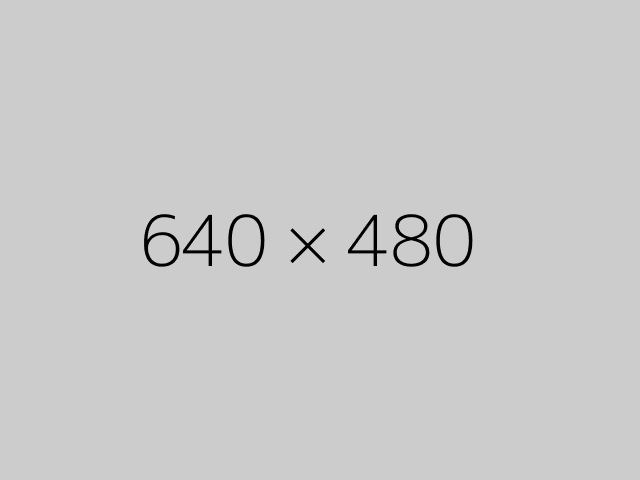
\includegraphics[width=0.6\textwidth]{dummy.png}
		}
		\center{\caption{BLEU on test set for transformer model by beam size}}
	\end{figure}
	
	Так же была обучена ансамбль из 5ти моделей с архитектурой \bibref{fconv}{Gehring et al.}{2017}, итоговые метрики для данного ансамбля можно видеть на изображении 8. Как можно видеть, трансформер показывает более высокие результаты, поэтому в качестве итоговой модели для экспериментов будем рассматривать именно трансформер.
	
	\begin{figure}[t]
		\center{
			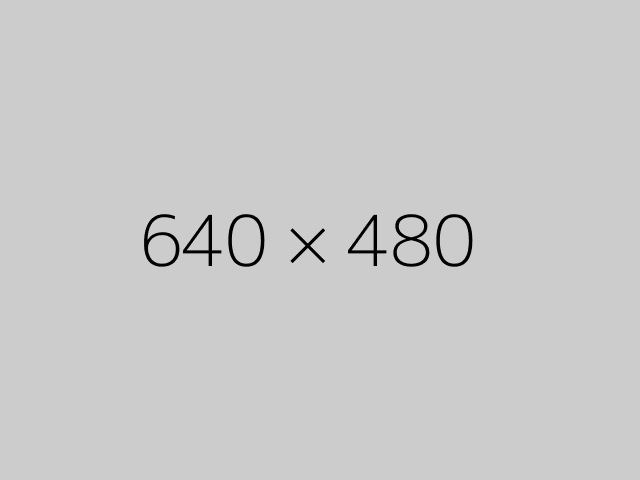
\includegraphics[width=0.6\textwidth]{dummy.png}
		}
		\center{\caption{BLEU on test set for fconv model by beam size}}
	\end{figure}
	
	Конфигурация каждой модели в ансамбле трансформеров была следующей:
	\begin{enumerate}
		\item $clip\_norm = 0$
		\item $learning\_rate=5*10^{-4}$
		\item $label\_smoothing=0.1$
		\item $epochs=75$
		\item $lenpen=0$ (Мы хотим знать как будут влиять uncertainty estimation на деградацию BLEU от  beam size)
	\end{enumerate}
	
	Из графиков итоговых метрик видно, что с ростом beam size BLEU деградирует. Как мы выяснили ранее, это может быть вызвано завышением или занижением вероятностей тех или иных токенов. В данной работе мы так же попробуем выявить корреляцию этой проблемы с оценкой неопределенности.
	
\section{Misclassification detection}
	В работе \bibref{uncertainty}{Malinin et al.}{2020} рассматривается попытка детекции ложно предсказанных токенов на задаче ASR. К сожалению, автор не проводил аналогичный эксперимент для NMT в связи с сложностью задания целевой метрики в машинном переводе.
	
	В нашей работе мы решили явно проверить, можно ли с помощью некоторых оценок неопределенностей обнаружить ошибочное предсказания очередного токена.
	
	Структура эксперимента будет следующей. Мы рассматриваем корпус предложений $X, R$. Пусть $y = (y^1, \dots, y^N)$ - соответствующие переводы, построенные ансамблем. Пусть $r_{i}, y_{i}$ - $ith$ токены истинного перевода и перевода модели, соответственно. Введем следующий индикатор корректности ith токена в переводе:
	\begin{equation}
		correct(y^{i}, \textbf{r}) := [y^{i} \in \textbf{r}]
	\end{equation}
	
	Данная индикаторная величина будет нашей целевой функцией, которую мы хотим предсказывать по оценке неопределенности. Введем теперь \textit{total uncertainty estimation}:
	\begin{equation}
		TU(y_i) := \mathcal{H}[P(y_i|y_{<i}, \mathcal{D})]
	\end{equation}
	
	Здесь в качестве $\mathcal{H}$ рассматривается энтропия по Шеннону. Данная метрика не разделяет виды неопределенностей, которые мы рассматривали ранее, она является индикатором для любого проявления. Она показывает насколько вероятностная масса итогового ансамбля разрежена по токенам словаря.
	
	Тогда для каждого токена $y_i^j \in H$ мы имеем целевывые функции $correct(y_i^j, r^j)$ и оценки неопределенностей $TU(y_i^j)$. Отнормируем на $[0, 1]$ оценки неопределенностей и получим некоторую модель, предсказывающую уверенность в ошибочности предсказания конкретного токена.
	
	\begin{figure}[t]
		\center{
			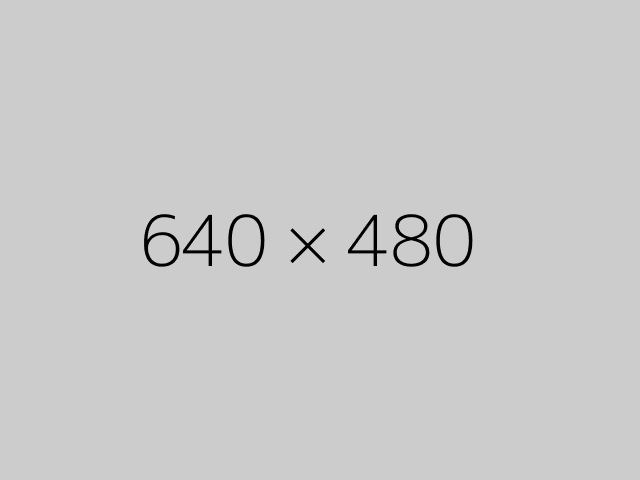
\includegraphics[width=0.6\textwidth]{dummy.png}
		}
		\center{\caption{PR-curve for misclassification detection by TU}}
	\end{figure}
	Результаты эксперимента можно видеть на изображении 9. Если мы пытаемся максимизировать F1-score, то показатели получились хуже, чем у случайного предсказателя, однако, если нас утроит отлов только маленькой доли ошибок, мы можем получить сравнительно неплохую точность детекции. 
	
	Результаты, полученные нами согласуются с тезисом, выдвинутым Малининым. Казалось бы, индикатор корректности мы зафиксировали очень свободный, ошибкой считается всякий токен, которого, вообще, нет в переводе, но при этом оценка неопределенностей работает хуже, чем случайное предсказание. Проблема кроется в том, что, если в качестве перевода выдан близкий по смыслу синоним, в котором модели ансамбля сильно уверены, то с точки зрения нашего индикатора - это ошибка, однака оценка неопределенностей не обнаружит никаких аномалий. Как было замечено Малининым в своей статье, решением проблемы будет ручная разметка данных людьми для выявления более осмысленных таргетов в данном эксперименте.
	
	Однако, мы все-таки попробуем некоторые другие подходы и попытаемся их сравнить с данным. Возможно, нам удасться, используя другие оценки или индикаторы похожести добиться более высокого качества.
	
	\textbf{TODO KL + DU}
	
	Давайте теперь проведем аналогичные эксперименты для нового индикатора корректности:
	\begin{equation}
		\delta(y^i, \textbf{r}) := [y^i = r^i]
	\end{equation}
	
		
	\begin{figure}[t]
		\center{
			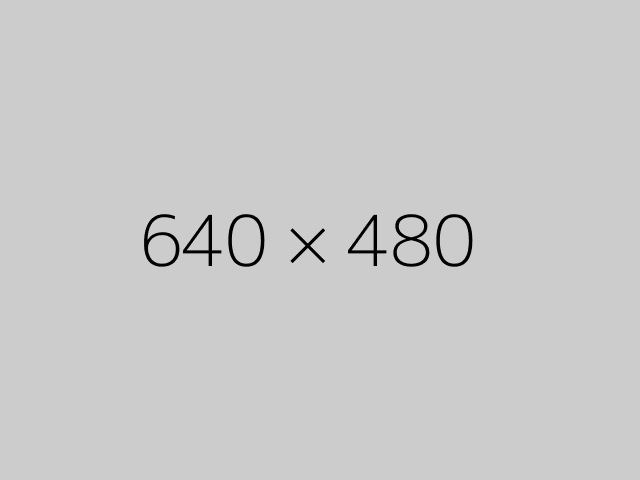
\includegraphics[width=0.6\textwidth]{dummy.png}
		}
		\center{\caption{PR-curve for misclassification detection by TU. $\delta(y^i, \textbf{r})$}}
	\end{figure}	
	И рассмотрим результаты на изображении 10. В этот раз наблюдаются очень высокие показатели. Однако, вызваны они не тем, что мы подобрали более релевантный индикатор корректности, а тем, что этот индикатор более строго определяет понятие ошибки. Теперь более вероятно встретить мисклассификацию и как следствие оценке неопределенностей легче стало с этим справляться. Поэтому данные результаты не очень resonable. Это легко видеть, если рассмотреть roc на изображении 11. Наша эмпирическая модель не сильно лучше справляется с задачей, чем случайный алгоритм. Важно заметить, после того как мы усилили условие корректности, доля положительного класса сильно выросла (0.76 против 0.26 в предыдущей постановке). Т.е. в данной постановке мы можем доверять ROC, поскольку положительный класс преобладает и как следствие баланс классов не ухудшает показатели.
	
	\textbf{TODO KL + DU}
	
	\textbf{Пассаж про beam size}

	\begin{figure}[t]
		\center{
			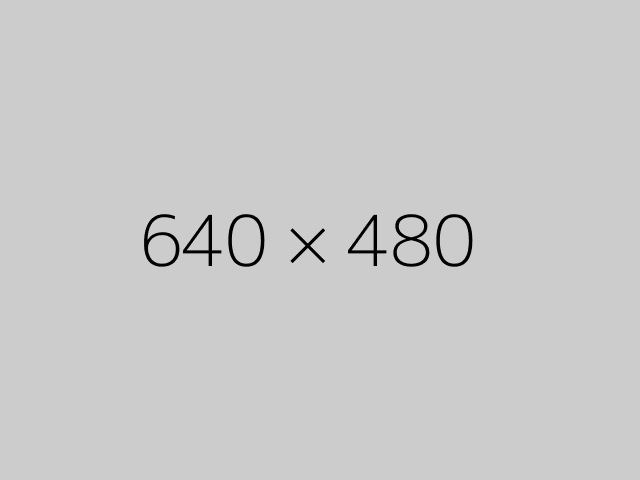
\includegraphics[width=0.6\textwidth]{dummy.png}
		}
		\center{\caption{ROC for misclassification detection by TU. $\delta(y^i, \textbf{r})$}}
	\end{figure}
	
\section{Корректность эксперимента}
	Возникает важный вопрос: почему в принципе ошибка классификации может коррелировать с оценкой неопределенности TU. Попробуем ответить на этот вопрос.
	
	\begin{figure}[t]
		\center{
			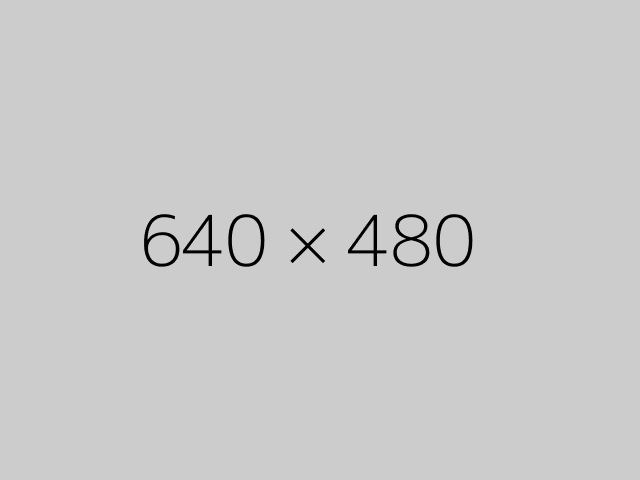
\includegraphics[width=0.6\textwidth]{dummy.png}
		}
		\center{\caption{Ensemble softmax Shannon entropy}}
	\end{figure}
	
	Попробуем оценить плотность распределения энтропии softmax для двух случаев: мы верно предсказали токен и мы допустили первую ошибку в предложении (весь префикс до этого токена мы предсказали верно). Т.е. для каждого такого случая мы посчитаем энтропию софтмакса и построим эмпирические оценки плотностей (отнормированные гистограммы). Результаты можно наблюдать на изображении 12.
	
	Как мы можем видеть, плотности в обоих случаях распределены почти нормально, унимодально. Причем мода распределения энтропий корректных токенов лежит строго левее моды распределения для первой ошибки, т.е. бОльшая часть вероятностной массы корректных токенов имеет более низкую энтропию у софтмакса (метрика TU). 
	
	Как мы можем это интерпретировать? Чем выше энтропия распределения, тем распределение более приближено к равномерному, т.е. все больше и больше появляются конкурирующих гипотез, т.е. наш ансамбль выделяет больше и больше равновероятных вариантов, а именно менее уверен в своем ответе. И наоборот если энтропия очень низкая, то распределение приближено к вырожденному, т.е. одна гипотеза имеет около единичную уверенность с точки зрения ансамбля. 
	
	Таким образом, если TU достаточно велико, это может быть индикатором того, что мы не очень уверены в токене, который мы предсказываем, что и позволяет нам оценить неопределенность в выставлении ответа.
	
	\textbf{TODO KL + DU + Beam size}
	
\section{Как использовать это на практике}
	Предположим, что мы смогли добиться внушительных показателей, построив некоторую оценку неопределенности $PerfectTU$. Как мы могли бы это использовать для улучшения качества?
	
	К сожалению, возможностей не так много. Все, что мы можем сделать - это помечать в предложениях позиции, на которых мы ошибаемся, и, как следствие, менять наши предсказания. В силу консистентности моделей машинного перевода, было бы логично строить перепрогноз не на основе исходной модели, а обращаться к некоторому оракулу, который выдает более надежные предсказания. На практике, таким оракулом мог быть некоторый ассессор или модератор. Однако, данный подход накладывает сильные ограничения на возможности использования оценки неопределенности, т.к. не всякий проект может позволить поддержку человеческих ресурсов. Более того, если в задаче необходимо выдавать быстрые онлайн предсказания, использование модераторов становится невозможным.
	
	Таким образом, мы приходим к необходимости поменять способ оценивания неопределенности. Нам необходимо найти такой способ оценивания, чтобы наша модель смогла сама на основе оценки неопределенности поменять предсказания. На данный момент это невозможно сделать, т.к. предсказываемые токены при фиксированном префиксе имеют одну и ту же оценку неопределенности. В качестве нашего следующего подхода мы будем строить оценки не для всего софтмакса сразу, а для каждого токена в софтмаксе отдельно.
	
	В предыдущих разделах мы рассматривали KL в качестве оценки knowledge uncertainty. Давайте введем метрику, которая будет коррелировать с KL, но при этом будет строиться для каждого токена.

\section{Inensemble variance}
	Напомним, что для каждого токена у нас определена вероятность:
	\begin{equation*}
		P(y_i | y_{<i}, x, \mathcal{D}) = \frac1{K} \sum_{j=1}^{K}P(y_i | y_{<i}, x, \theta_j)
	\end{equation*}
	
	Таким образом, для каждого токена мы имеем: условную вероятность токена для ансамбля и K условных вероятностей токена для моделей. Давайте в качестве меры неопределенности введем несмещенную выборочную дисперсию токена вдоль моделей в ансамбле:
	\begin{equation}
		inens\_var(y_i) := S^2(P(y_i | y_{<i}, x, \theta_1), \dots, P(y_i | y_{<i}, x, \theta_K))
	\end{equation}
	
	Данная оценка будет служить мерой согласованности моделей в предсказании вероятности данного токена (некоторый аналог KL в предыдущих главах). Заметим, что энтропийный критерий более подходит для нас в качестве меры неопределенности, т.к. с помощью дисперсии сложно разделять случаи: вырожденное распределение и равномерное распределение. Тем не менее, дисперсия все еще позволяет отделить распределения с высоким уровнем конкурирующих гипотез. Мы остановились на выборе именно дисперсии, т.к. вероятности моделей не образуют вероятностную меру (на этих вероятностях не задано распределение, значения могут быть абсолютно не согласованными), поэтому вычисление энтропии некорректно в данном случае.
	
	\begin{figure}[t]
		\center{
			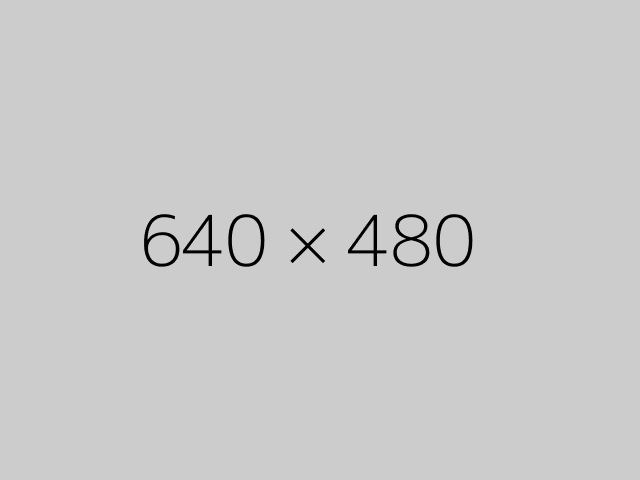
\includegraphics[width=0.6\textwidth]{dummy.png}
		}
		\center{\caption{Inensemble variance among models for correct token and first error token}}
	\end{figure}
	Рассмотрим следующий график (изображение 13). Здесь представлена плотности новой оценки неопределенности для двух видов токенов: первый ошибочный токен в предложении (префикс до этого токена предсказали корректно) и истинный токен для этой позиции при том же префиксе. Сразу можно заметить, что как и в предыдущем случае бОльшая часть вероятностной массы корректного токена находится на порядки левее (меньшая дисперсия), чем у ошибочного токена. Данное наблюдение дает нам надежду на то, что модели в ансамбле выдают более согласованные предсказания вероятностей для корректного токена и больше сомневаются в выставленной вероятности для итогового токена.
	
	Возникает закономерный вопрос: почему несмотря на более низкую согласованность, в итоговом предсказании оказался тот токен, который оказался. Для ответа на данный вопрос нам необходимо посмотреть на распределения вероятностей для этих же токенов (изображение 14).
	
	\begin{figure}[t]
		\center{
			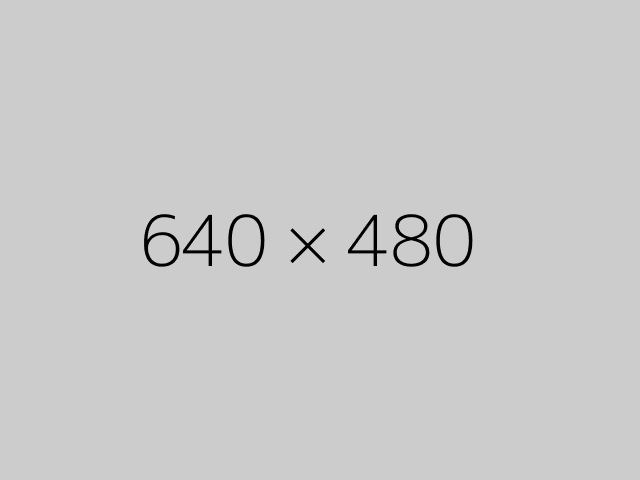
\includegraphics[width=0.6\textwidth]{dummy.png}
		}
		\center{\caption{Token-level ensemble probability for correct token and first error token}}
	\end{figure}
	
	Как мы видим из графиков, мы допускаем ошибку на данной позиции, т.к. зачастую мы имеем около нулевую вероятность для истинного токена, поэтому отдается предпочтение более вероятному токену (и его продолжению).
	
	\begin{figure}[t]
		\center{
			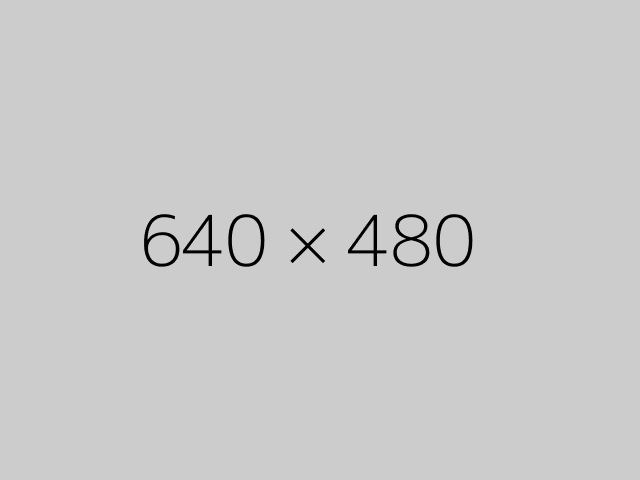
\includegraphics[width=0.6\textwidth]{dummy.png}
		}
		\center{\caption{Token-level ensemble probability by inensemble variance for correct token and first error token}}
	\end{figure}
	Так же хотелось бы взглянуть как соотносятся между собой значения дисперсий и значения вероятностей. Перейдем к графику 15. В данном графике раскрывается серьезный недостаток рассмотрения дисперсии. Рассмотрим следующий пример. Пусть мы имеем некоторую выборку $t = (t_1, \dots, t_m)$ и пусть ей соответсвует выборочное среднее: $S^2(t)$. Вычислим:
	\begin{equation*}
		S^2(\alpha t) = S^2((\alpha t_1, \dots, \alpha t_m)) = \alpha^2 S^2(t)
	\end{equation*}
	
	Таким образом, значение нашей метрики зависит не только от совокупного соотношения величин в выборке, но и от порядка этих значений. Именно этот эффект мы и наблюдали на графике 15. Для бОльшей вероятностной массы корректного токена низкое значение оценки неопределенности которую мы выбрали вызвано не согласованностью моделей, а порядком вероятности, т.е. дисперсия около нулевых вероятностей засчет свойства выше на порядки ниже всегда.
	
	Однако, несмотря на это, сопоставляя дисперсии корректного и ошибочного токена при равных вероятностях, мы можем наблюдать, что ожидаемая дисперсия для корректного токена выше, чем для ошибочного. Поэтому хотя и не на всей вероятностной массе, но на некоторой ее адекватной части наша оценка неопределенности дает адекватные предсказания.
	
	Для того, чтобы в этом убедиться, необходимо посмотреть как ведет себя наша оценка на других токенах этого же софтмакса. Для этого будем рассматривать: случайный токен, токены с топ-3, топ-5 и топ-20 вероятностями в вариационном ряду по убыванию. Итоговые графики распределения вероятностей и оценок неопределенностей можно видеть на фигуре 16.
	
	\begin{figure}[t]
		\center{
			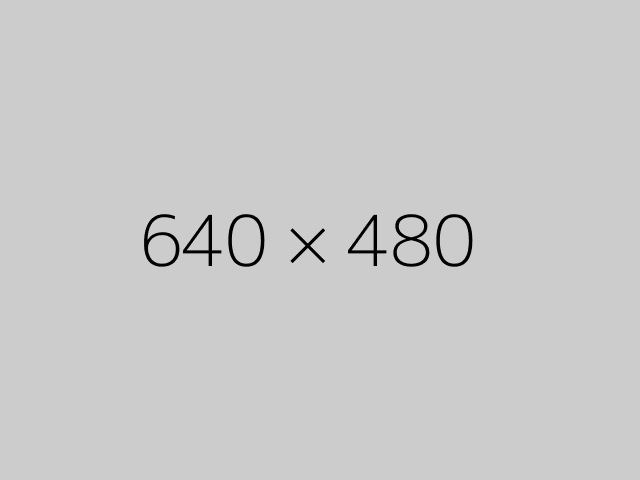
\includegraphics[width=0.6\textwidth]{dummy.png}
		}
		\center{\caption{Token-level ensemble probability and inensemble variance for correct token, first error token, random token, top-3 top-5 and top-20 tokens}}
	\end{figure}
	
	Как мы видим, корректные токены не такие безнадежные. Высокая доля вероятностной массы корректных токенов имеет сравнительно высокие вероятности (ожидаемая позиция в вариационном ряду вероятностей == 2). Более того уверенность моделей в корректных токенах разительно не уступает дисперсии других токенов. Мы можем воспользоваться данными наблюдениями, чтобы помочь модели находить корректные токены.
	
\section{Перевзес вероятностного распределения}
	Наша задача сейчас перенормировать метрикой неопределенности вероятностные распределения токенов таким образом, чтобы распределение корректного токена стало более превалирующим с точки зрения выбора итоговой гипотезы моделью. Таким образом, задача сводится к нахождению некоторой функции $g$:
	\begin{equation*}
		\hat{p}(y | x, \mathcal{D}) = softmax(g(p(y | x, \mathcal{D}),\, inens\_var(y)))
	\end{equation*}
	
	Если мы посмотрим на график 17, то станет ясно, что подбором $g$ мы можем искривлять этот график только вдоль оси X. Говоря наглядным языком, мы бы хотели вдоль каждой линии уровня дисперсии стянуть плотность корректного токена к правому краю, а плотность всякого любого другого токена к левому.
	
	\begin{figure}[t]
		\center{
			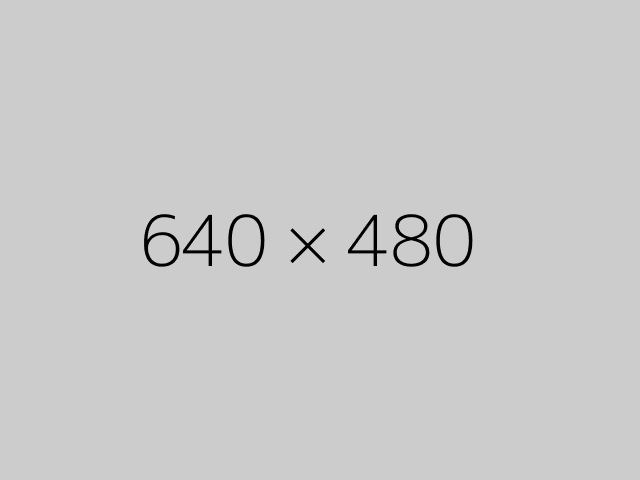
\includegraphics[width=0.6\textwidth]{dummy.png}
		}
		\center{\caption{Token-level ensemble probability by inensemble variance for correct token, first error token, random token, top-3 top-5 and top-20 tokens}}
	\end{figure} 
	
	Напомним, что мы бы хотели штрафовать за высокие значения uncertainty, однако не так сильно, чтобы не перевзвесить совсем нерелевантные токены. Плохим примером функции $g$ будет:
	Здесь и далее положим: $\sigma^2 := inens\_var$
	\begin{equation}
		g_{naive} := \log p(y | x, \mathcal{D}) - \log(\sigma^2)
	\end{equation}
	
	Мы явно награждаем токены с очень низким значением дисперсии и, наоборот, сильно штрафуем за высокие значения неопределенности. Данный наивный подход приводит к диаметрально противоположной ситуации (изображение 18). Мы, видим, что такие сильные штрафы приводят к тому, что высокую вероятность принимаю не осмысленные токены, а случайные. Это происходит по той причине, что дисперсия случайных токенов крайне низка из-за особенностей метрики, которые мы обсуждали ранее. В итоге модель просто выдает абсолютно случайные переводы.
	
	\begin{figure}[t]
		\center{
			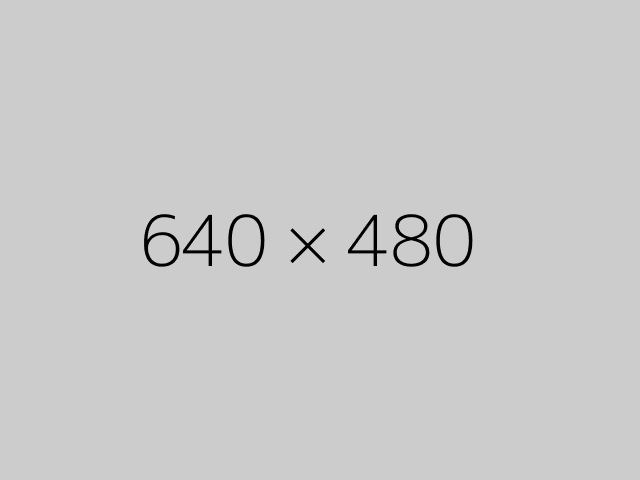
\includegraphics[width=0.6\textwidth]{dummy.png}
		}
		\center{\caption{Token-level ensemble probability by inensemble variance for correct token, first error token, random token, top-3 top-5 and top-20 tokens}}
	\end{figure}
	
	Попробуем несколько ослабить штраф за неопределенность, делить вероятность на коррень из меры неопределенности:
	\begin{equation}
		g_{less\_naive} := \log p(y | x, \mathcal{D}) - \log(\sigma)
	\end{equation}
	
	Как мы видим из графика 19, это не привнесло никаких успехов, т.к. мы не поменяли даже относительный порядок распределений вероятностей.
	
	Если мы еще раз взглянем на график 17, то будет ясно, что линейными функциями $g$ мы не сможем добиться перестройки порядка следования распределений с точки зрения вероятностей (напомним, что график представлен в лог шкалах). Таким образом, мы приходим к тому, что преобразование должно быть не линейным по $\log \sigma^2$, более того пик (точка максимума) должна приходиться на кусок распределения корректного токена, который не перекрывается никаким другим распределением.
	
	Тогда давайте в качестве такой функции возьмем:
	\begin{equation}
		g_{2} := \log p(y | x, \mathcal{D}) - (\log(\sigma) + \alpha)^2
	\end{equation}
	
	 Где $\alpha$ некоторый гиперпараметр, от которого будет зависеть в какой точке будет достигаться максимум. Рассмотрим частный пример (график 20).
	 
	 \begin{figure}[t]
		\center{
			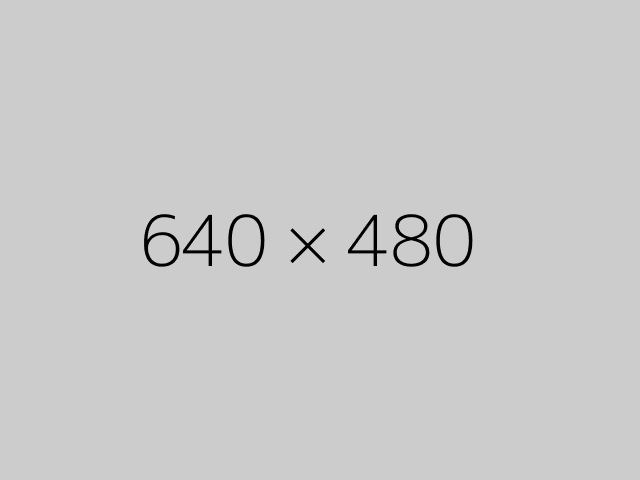
\includegraphics[width=0.6\textwidth]{dummy.png}
		}
		\center{\caption{Token-level $softmax(g_2)$ by inensemble variance for correct token, first error token, random token, top-3 top-5 and top-20 tokens}}
	\end{figure}
	
	\textbf{TODO}
	
	Заметим, что плотность ошибочного токена по прежнему осталась правее, плотности корректного токена. К сожалению или к счастью, с этими точками мы не можем ничего сделать, т.к. если на одной и той же линии уровня дисперсий некоторый токен имеет бОльшую вероятность, очевидно, мы должны отдавать предпочтение именно этому токену. Однако, даже уже полученные результаты могут привести к неплохим результатам, т.к. в случае не единичиного beam size даже небольшой перевзвес может привести к выбору корректных гипотез, т.к. выбор гипотезы делается на основе куммулятивных вероятностей, а не на основе жадного выбора.
\section{BLEU перезвеса}
	\textbf{TODO}
	
\section{Выводы}
	\textbf{TODO}
	
	
	

	\begin{thebibliography}{0}		
		\bibitem{fconv}\hypertarget{fconv}{}
		\href{https://arxiv.org/pdf/1705.03122.pdf}
		{Jonas Gehring, Michael Auli, David Grangier, Denis Yarats, Yann N. Dauphin. Facebook AI Research. Convolutional Sequence to Sequence Learning. PMLR 70, 2017.}
		
		\bibitem{seq2seq}\hypertarget{seq2seq}{}
		\href{https://papers.nips.cc/paper/5346-sequence-to-sequence-learning-with-neural-networks.pdf}
		{Ilya Sutskever, Oriol Vinyals, Quoc V.Le. Sequence to Sequence Learning with Neural Networks. Google. NIPS 2014.}
		
		\bibitem{encdec_att}\hypertarget{encdec_att}{}
		\href{https://arxiv.org/pdf/1409.0473.pdf}
		{Dzmitry Bahdanau, KyungHyun Cho, Yoshua Bengio. Neural Machine Translation by Jointly Learning to Align and Translate. ICLR 2015.}
		
		\bibitem{corr_len_bias}\hypertarget{corr_len_bias}{}
		\href{https://arxiv.org/pdf/1808.10006.pdf}
		{Kenton Murray, David Chiang. Department of Computer Science and Engineering, University of Notre Dame. Correcting Length Bias in Neural Machine Translation. WMT 2018.}
		
		\bibitem{gnmt}\hypertarget{gnmt}{}
		\href{https://arxiv.org/pdf/1609.08144.pdf}
		{Yonghui Wu, Mike Schuster, Zhifeng Chen, Quoc V. Le, Mohammad Norouzi. Google’s Neural Machine Translation System: Bridging the Gapbetween Human and Machine Translation. ArXiv 2016}
		
		\bibitem{transformer}\hypertarget{transformer}{}
		\href{https://arxiv.org/pdf/1706.03762.pdf}
		{Ashish Vaswani, Noam Shazeer, Niki Parmar, Jakob Uszkoreit, Llion Jones, Aidan N. Gomez, Lukasz Kaiser. Attention Is All You Need. NIPS 2017.}
		
		\bibitem{six_chall}\hypertarget{six_chall}{}
		\href{https://arxiv.org/pdf/1706.03872.pdf}
		{Philipp Koehn, Rebecca Knowles. Six Challenges for Neural Machine Translation. NMT@ACL 2017.}
		
		\bibitem{calibration}\hypertarget{calibration}{}
		\href{https://arxiv.org/pdf/1903.00802v1.pdf}
		{Aviral Kumar, Sunita Sarawagi. Calibration of Encoder Decoder Models for Neural Machine Translation. ArXiv 2019.}
		
		\bibitem{anal_uncertainty}\hypertarget{anal_uncertainty}{}
		\href{https://arxiv.org/pdf/1803.00047.pdf}
		{Myle Ott, Michael Auli, David Grangier, Marc'Aurelio Ranzato. Analyzing Uncertainty in Neural Machine Translation. PMLR 80, 2018.}
		
		\bibitem{prior}\hypertarget{prior}{}
		\href{https://papers.nips.cc/paper/7936-predictive-uncertainty-estimation-via-prior-networks.pdf}
		{Andrey Malinin, Mark Gales. Predictive Uncertainty Estimation via Prior Networks. NeurIPS 2018.}
		
		\bibitem{uncertainty}\hypertarget{uncertainty}{}
		\href{https://arxiv.org/pdf/2002.07650.pdf}
		{Andrey Malinin, Mark Gales. Uncertainty in Structured Prediction. 2020.}
	\end{thebibliography}


\end{document}

